\documentclass[10pt]{article}
% \usepackage[margin=1in]{geometry}
% \newcommand\hmmax{0}
% \newcommand\bmmax{0}
% % % Fonts% %
\usepackage{luatexja}

\usepackage[T1]{fontenc}
   % \usepackage{textcomp}
   % \usepackage{newtxtext}
   % \renewcommand\rmdefault{Pym} %\usepackage{mathptmx} %\usepackage{times}
\usepackage[complete, subscriptcorrection, slantedGreek, mtpfrak, mtpbb, mtpcal]{mtpro2}
   \usepackage{bm}% Access to bold math symbols
   % \usepackage[onlytext]{MinionPro}
   \usepackage[no-math]{fontspec}
   \defaultfontfeatures{Ligatures=TeX,Numbers={Proportional}}
   \newfontfeature{Microtype}{protrusion=default;expansion=default;}
   \setmainfont[Ligatures=TeX]{Source Serif Pro}
   \setsansfont[Microtype,Scale=MatchLowercase,Ligatures=TeX,BoldFont={* Semibold}]{Source Sans Pro}
   \setmonofont[Scale=0.8]{Atlas Typewriter}
   % \usepackage{selnolig}% For suppressing certain typographic ligatures automatically
   \usepackage{microtype}
% % % % % % %
\usepackage{amsthm}         % (in part) For the defined environments
\usepackage{mathtools}      % Improves  on amsmaths/mtpro2
\usepackage{amsthm}         % (in part) For the defined environments
\usepackage{mathtools}      % Improves on amsmaths/mtpro2
\usepackage{xfrac}

% % % The bibliography % % %
\usepackage[backend=biber,
  style=authoryear-comp,
  bibstyle=authoryear,
  citestyle=authoryear-comp,
  uniquename=false,%allinit,
  % giveninits=true,
  backref=false,
  hyperref=true,
  url=false,
  isbn=false,
  useprefix=true,
  ]{biblatex}
\DeclareFieldFormat{postnote}{#1}
\DeclareFieldFormat{multipostnote}{#1}
% \setlength\bibitemsep{1.5\itemsep}
\newcommand{\noopsort}[1]{}
\addbibresource{Thesis.bib}

% % % % % % % % % % % % % % %

\usepackage[inline]{enumitem}
\setlist[itemize]{noitemsep}
\setlist[description]{style=unboxed,leftmargin=\parindent,labelindent=\parindent,font=\normalfont\space}
\setlist[enumerate]{noitemsep}

% % % Misc packages % % %
\usepackage{setspace}
% \usepackage{refcheck} % Can be used for checking references
% \usepackage{lineno}   % For line numbers
% \usepackage{hyphenat} % For \hyp{} hyphenation command, and general hyphenation stuff
\usepackage{subcaption}
% % % % % % % % % % % % %

% % % Red Math % % %
\usepackage[usenames, dvipsnames]{xcolor}
% \usepackage{everysel}
% \EverySelectfont{\color{black}}
% \everymath{\color{red}}
% \everydisplay{\color{black}}
\definecolor{fuchsia}{HTML}{FE4164}%Neon Fuchsia %{F535AA}%Neon Pink
% % % % % % % % % %

\usepackage{pifont}
\newcommand{\hand}{\ding{43}}
\usepackage{array}


\usepackage{multirow}
\usepackage{adjustbox}

\usepackage{titlesec}

\makeatletter
\newcommand{\clabel}[2]{%
   \protected@write \@auxout {}{\string \newlabel {#1}{{#2}{\thepage}{#2}{#1}{}} }%
   \hypertarget{#1}{#2}
}
\makeatother

\usepackage{multicol}

\setcounter{secnumdepth}{4}
\setcounter{tocdepth}{4}

\usepackage{tikz}
\usetikzlibrary{bending,arrows,positioning,calc}
\usepackage{tikz-qtree} %for simple tree syntax
% \usepgflibrary{arrows} %for arrow endings
% \usetikzlibrary{positioning,shapes.multipart} %for structured nodes
\usetikzlibrary{tikzmark}
\usetikzlibrary{patterns}


\usepackage{graphicx} % for images (png/jpeg etc.)
\usepackage{caption} % for \caption* command


\usepackage{tabularx}

\usepackage{bussalt}

\usepackage{Oblique} % Custom package for oblique commands
\usepackage{CustomTheorems}

\usepackage{svg}
\usepackage[off]{svg-extract}
\svgsetup{clean=true}



\usepackage{dashrule}

\newcommand{\hozline}[0]{%
  \noindent\hdashrule[0.5ex][c]{\textwidth}{.1pt}{}
  %\vspace{-10pt}
  % \noindent\rule{\textwidth}{.1pt}
}

\newcommand{\hozlinedash}[0]{%
  \noindent\hdashrule[0.5ex][c]{\textwidth}{.1pt}{2.5pt}
  %\vspace{-10pt}
}

\usepackage{contour}
% \usepackage{pdfrender}

\usepackage{extarrows}

\usepackage[hidelinks,breaklinks]{hyperref}

\title{Means-end reasoning and means-end relations}
\author{Ben Sparkes}
% \date{ }


\begin{document}

% How to like cases in which an agent responds to reasons that they do not grasp.

\section{Motivation}
\label{sec:motivation}

At present, this motivation is intrinsic.
There are few hints in the literature, but nothing developed in significant detail.
So, the idea and how it can be used to understand phenomena.

\begin{itemize}
\item Present the basic case.
\item Analysis, features.
\item Outline two other cases.
\item Discussion.
\end{itemize}

\section{Introduction}
\label{sec:introduction}

Provide cases in which an agent responds to reasons that the agent is confident that they possess without the agent understanding how they are responding to the possessed reasons.

These cases involve the adoption of an attitude toward some proposition.

In each case the agent is confident that they hold some collection of attitudes, and that the collection of attitudes supports adopting a further attitude toward a further proposition.

Quick example.
Shopping list.
Item on the shopping list, but the agent cannot recall why they put the item on the shopping list.
Agent is confident that they continue to hold the attitudes which support purchasing the item, but cannot recall what these are.
The shopping list provides information about what follows from those attitudes, the particular item.
Hence, the agent purchases the item, confident that they are responding to reasons generated by the attitudes they possess without understanding how purchasing the item responds to those reasons.

The term `reasons' is used loosely here, as attitudes may not generate genuine reasons.

The main issue is whether the information that details what follows from the attitudes that the agent assumes they possess (the shopping list) combines with some other attitudes of the agent to rationalise their behaviour.
It may be that I have a collection of attitudes that support purchasing whatever is listed on my shopping list, and this collection of attitudes is accessible and independent from those attitudes which supported placing any given item on the list.

Main case will be epistemic.
There's some bite only when something is done on the basis of these attitudes, but epistemologists have some very nice tools.

In the type of cases I will construct, \dots
\begin{itemize}
\item Agent is confident that they have a certain collection of attitudes
\item Agent has support that a certain attitude toward a proposition follows from that collection of attitudes.
\item This will not rule out other explanations.
\item Quite weak.
\item Difficulty is motivating the role of the attitudes.
\item Key here is different kind of support, between attitudes and evidence.
\item Fail to respond, or fail to respond by understanding.
\item Difference, and if these can come apart then can expect agent to sometimes respond without understanding.
\item Of course, also expect agent not to respond without understanding, but this is for another time.
\item Responding to reasons literature, Worsnip, Lord.
\item Alternatively, different attitudes (Buchak, etc.), \dots
\end{itemize}

So it is with the philosophy of action.
Start with a epistemic interpersonal case, and then show how this can be transformed into a desire intrapersonal case.

Not clear that the agent is rational.
It seems clear the agent is not ideally rational, as the case rely on the agent lacking access to attitudes they have.
Issue is whether the agent is responding to rational pressures, even if unsuccessfully, in the way that one slowly moves backwards while walking on a treadmill set at pace which is slightly too high for one's gait.

\section{The Basics}
\label{sec:basics}

\begin{itemize}
\item Support
  \begin{itemize}
  \item Or justification.
  \item Two aspects.
    \begin{itemize}
    \item Constructive vs.\ non-constructive
    \item Hypothetical vs.\ categorical
    \end{itemize}
  \end{itemize}
\end{itemize}

\begin{itemize}
\item Support for a proposition establishes a proposition (in some way).
\item Whether the proposition is true, worthwhile, believed, desired, and so on.
\item In the chess scenario, the proposition is that there is a winning strategy.
\item In the Morse scenario, the proposition is that a certain person is guilty.
\item In the shopping example, the proposition is that a certain item is worthwhile.
\end{itemize}

\begin{itemize}
\item Distinction between constructive and non-constructive support.
\end{itemize}

\begin{itemize}
\item In the scenario there is some property proposition which has a property.
\item It is true that there is a winning strategy given the state of the board and the rules of chess.
\item It may also be beneficial that there is a winning strategy given the state of the board and the rules of chess, and so on.
\item Important that the property does not required constructive support --- does not depend on a witness.
  \begin{itemize}
  \item In the cases of interest, the witness is provided by the agent's reasoning.
  \item So, could say that the property does not depend on reasoning.
  \item However, agent's confidence is supported by previous instance of reasoning.
  \item Given a broad account of properties, the reasoning could be the required witness.
  \item For example, inferred belief.
  \item Agent is confident that they inferred the truth of some proposition and believe the proposition given reasoning.
  \item Agent cannot recall the reasoning, but remains confident that they did infer the proposition.
  \item Narrowing to present reasoning may avoid this problem, but if you're willing to push hard on edge cases then there may be instances of the agent's reasoning being inaccessible as in two-stage models of cognition.
  \item In short, relying on an intuitive concept of a witness is not particularly informative, but providing a analysis of this concept raises issues which go beyond the core type of scenario.
   % \item Ironically, then, by failing to provided a witnessing concept of constructive support I have not provided constructive support for constructive support, so be it.
  \end{itemize}
\end{itemize}
Truth is a nice example.
Seeing or entertaining won't work.\nolinebreak
\footnote{
  Well, except in cases of co-reference.
  Here, there are all sorts of things that can be Done.
}
\begin{itemize}
\item A winning strategy for a game of chess does not depend on an agent reasoning to that winning strategy.
\end{itemize}




\begin{itemize}
\item Accessibility.
\end{itemize}

\section{Support}
\label{sec:support}

\begin{note}
  This comes after the main case.
\end{note}

\begin{itemize}
\item Categorical and hypothetical
\item Constructive and non-constructive
\end{itemize}


Legal distinction between statistical, direct, and circumstantial evidence.
Direct evidence isn't quite right, as with direct evidence no intervening inference can be required.
Circumstantial evidence does require inference, but this is tied to the idea of reasonable doubt.
There is no need to rely on legal terminology.
Instead, borrow from mathematics and talk of \emph{constructive} evidence.
Support is built from possessed information, and does not rely on appeal to any additional information.\nolinebreak
\footnote{
  Might think this gets difficult in the practical case, but I'm not so sure.
  What's worthwhile is determined by the attitudes an agent has, and so is constructed on the basis of these.
  So I'm assuming that this kind of reasoning is constructive in the relevant sense, if I think there are straightforward parallels.
  I think it's okay though, as it's basically tying the support to the information that the agent has.
}

Not too interested in proposition versus doxastic justification.
It is the case that there's something of interest here.
In particular, failure of doxastic justification for the belief that there is a winning strategy given the state of the board and the agent's grasp of the rules of chess.
However, this points out the obvious, and the issue is about what going on with the agent regardless of this failure of doxastic justification.

\subsection{Categorical and hypothetical}
\label{sec:categ-hypoth}

Following \textcite{Pryor:2018aa}.
Benefits of overloaded terminology.

Very much related to substantive and structural, as \citeauthor{Pryor:2018aa} notes.

\subsection{Constructive and non-constructive support}
\label{sec:constr-non-constr}


\begin{itemize}
\item Propositions
  \begin{itemize}
  \item Interpretation
  \item Reference
  \end{itemize}
\item Relation of support between propositions
  \begin{itemize}
  \item Binding
  \item Interim proposition
  \end{itemize}
\item Supporting proposition
  \begin{itemize}
  \item Constructive
  \item Non-constructive
  \end{itemize}
\end{itemize}


\[\exists x(WSx)\]

Proposition.
Refers when paired with an interpretation.
Agent understands what it means for there to be a winning strategy, but the agent doesn't have an interpretation.

Support.
Past experience, similarity to previous boards.
The support is complex.
Past experiences, present seemings, and broad principles.
Past experiences and present seemings are situations, and the agent refers to these by interpreting propositions.
Principles offer a guarantee that there is an extension of the agent's interpretation function to the proposition that a winning strategy exists, that this can refer to a situation (in particular the situation consisting of the winning strategy).
However, don't show how to extend the agent's interpretation function.

Contrast constructive with non-constructive support.
Support here is a many-to-one relation between premise propositions, some principles, and a target proposition.
\(\Phi \vDash_{I} \psi\).
Constructive if this extends the interpretation.
Non-constructive if it does not.

Hypothetical and categorical, about guaranteeing an interpretation.
Hypothetical is a conditional guarantee of interpretation.
Categorical is an unconditional guarantee of interpretation.

Agent, based on interaction with companion has good categorical non-constructive support for the existence of a winning strategy.
Agent, based on abilities has hypothetical constructive support for the existence of a winning strategy.
And, that the hypothetical constructive support for the existence of a winning strategy can be transformed into categorical constructive support for the existence of a winning strategy.

These are the key distinctions.

\begin{note}
  This is subtle.
  With Morse and Lewis, the idea is that Morse's statement doesn't provide evidence, as it just tells Lewis what follows from the dossier.
  So, Morse isn't providing testimony that the person is guilty, on that the person's guilt follows from the dossier.
  Morse is stating a relation, not outright guilt.
  Hence, Lewis has hypothetical constructive support, and this can be turned into categorical constructive support.

  If Lewis didn't have the dossier, things would be different, it seems.
  There's something about Lewis having a collection of reasons, and the same reasons that Morse is appealing to.
  So, Morse can't be providing additional reasons.
  And that's something of the puzzle.
  If Lewis didn't have the dossier, or Morse mentioned some new piece of information.

  So, the appeal to reasons is constructive or non-constructive.
  So, the distinction is easy to draw out in the chess example, because the proposition marks the difference.
  However, it's not the interpretation of the proposition that's important, it's how this is found.
  This gets back to responding to reasons.

  So, this is now quite different to the bus case.
  Well, except in the observation that with the witness testimony there's a constructive route.

  So, constructive/non-constructive is simple in the chess scenario.
  Can see that the support is non-constructive, that it doesn't explain \emph{why} there's a winning strategy.
  In the Lewis scenario, there's no existential, but it remains the case that there's something non-constructive, as there's no account of why the person is guilty.
  The point is that there's some stuff that the agent can use, and the way in which interpretation is fixed is important.

  Appealing to Morse, and using testimony in general, simply hands off this procedure to someone else.
  In this sense, there is an issue in that there's no clear line.
  Lewis, with the evidence, still relies on handing off, so the issue isn't about having an effective procedure, it's about taking a non-constructive route.
  The idea, then, is that one wants this to be as constructive as possible.
  That's the basic intuition.

  The key idea, I think, is that the agent, with constructive reference, establishes a link.
  The agent sees how the supporting propositions determine the target proposition, and if the supporting propositions are interpreted, how the interpretation of these is transformed to provide an interpretation of the target proposition.
  And, in a sense, this is a better state, as if there is a link then these things aren't independent.
  \(A, B, A \rightarrow B\) is better than \(A, B\).
\end{note}

\begin{note}
  Framing things in this way, it's certainly not clear that constructivity is desirable in general, which is nice.
\end{note}

\begin{note}
  In the case of buses, there's a way to fill in the existential, somehow.
\end{note}

\begin{note}
  This doesn't depend too much on structural issues.
  Key is constructing, and in this sense structural rationality is nice, because it doesn't make any demands on the agent.
  However, one could wiggle this a little, and still how that the agent has a requirement.
  So, there's potentially some overlap.
\end{note}

\begin{note}
  Parallels to constructive mathematics, but these are hard, as things bottom out in the real case, and it's not clear how much the mathematical arguments extend to cases where there's no pure constructive proof.
  And, as seen, easy to find non-constructive cases where there's no trouble with reference.
\end{note}

\begin{note}
  Appeal to something constructive is nice, as the constructiveness is an additional property.
  That is, there's something fine about the attitude even if it is not constructive.
\end{note}

\begin{note}
  Predictive power of this approach seems like it may be limited.
  For, in the case of mathematics it's not clear that there's much pressure for constructive proofs.
  Is there?
  This seems like a fairly decent objection, if there's not.

  So, this is an objection highlighting that there's no general argument for a constructive approach.
  Hence, there's going to be something about the circumstances that push toward a constructive approach.
  This, then, is a little bit of progress, as there's a contrast case.
  That is, in the case of constructive mathematics, there's potential, but it doesn't seem like a requirement to the same extent.
  This is likely true even if the agent has constructive foundations available to them.

  Distinguishing feature is that the agent wants to do something with the reference.
  The agent wants to observe the winning strategy.
  Lewis wants to arrest the person.
  The shopper wants to buy the ingredient.
  Without constructive reasoning, there's a gap allowing for the possibility that the reference isn't quite right.
  Or, something about the ability to determine the reference from the information that the agent has.
\end{note}

\begin{note}
  Demonstrate that the reference has some property, because something is done on the basis that the reference has the property.
  If non-constructive, then there's a missing link.
  No demonstration that the referent satisfies the property.
  Way to reason from the dossier to the guilt of \(a\), so here \(a\) is a witness to some implicit existential ``the criminal''.
  This is interesting, as could imagine that the companion gives the agent the strategy, still expect that there's some pressure for the agent to explore the possibilities, to ensure that they're ruled out.
\end{note}

\begin{note}
  Another mathematic example is certain calculations.
  There's no pressure on the agent to reason through the addition of some large numbers when a calculator does the job.
  Heck, even when I type some small numbers into the calculator there doesn't seem to anything particularly wrong.
  And this is a really interesting case for \citeauthor{Lord:2018aa}.
  However, a contrast here in that with addition the link is straightforward, there's no question about what the construction would look like, while in the cases in the scenario there is some question.
\end{note}


Smiley,
`There is a mole at the top of the circus'.
Two issues.
Whether there is evidence to support this, and who the mole is.

Write the proposition as

\[\exists x(Mx \land Cx)\]



The proposition is a way of representing a situation, and it does so by being paired with an interpretation function.


\[\exists x(Mx \land (x = a \lor x = b \lor x = c \lor x = d))\]

Familiar point, need an interpretation of \(a, b, c, d\) and most importantly there must be some object \(x\).
Smiley is able to refer to \(a, b, c, d\), but not to \(x\).
The presence of the variable is unimportant.
Simplify to:

\[Ma \lor Mb \lor Mc \lor Md\]

Smiley does not have an interpretation of \(Ma\).
Smiley is aware of the requirements of an interpretation of \(Ma\).
\(Ma\) is not meaningless, but it is not guaranteed to pick out a(n actual) situation.






Smiley gathers evidence, situations, and propositions which refer to these situations when paired with an adequate interpretation are shackled to the pages of a dossier by ink.
Smiley's interpretation is effective for some of these propositions, but for some it is not.
Testimony.
The evidence is the situation, and this passes through the witness.




`The mole whom Lapin serviced in London.'
`Gerald'
`Karla is the controller of Gerald'












Inspired by \textcite{Over:1983aa}.
The important thing here is the concept of \emph{effective reference}. (\cite{Over:1983ab})

\begin{quote}
  A speaker uses a singular term with effective reference if he associates with it an effective method of deciding whether any given object is its referent; otherwise the speaker uses the term with non-effective reference.\nolinebreak
  \mbox{}\hfill\mbox{(\citeyear[86]{Over:1983ab})}
\end{quote}

For \citeauthor{Over:1983ab}, effective reference concerns what an agent can do, not what an agent does and in this passage concerns singular terms.

Singular terms an a simple case.

For our purposes, broader understanding of effective reference.
Language and interpretation.
Able to identify or demonstrate what a proposition refers to.

This has little to do with support or evidence, for an agent may be able to determine what a proposition refers to without being in a position to establish whether what the proposition refers to is the case.
For example, working on identifying the ideal distribution of coffee shops in San Francisco.
Stack of partial maps, not sure whether the coffee shop is proposed or real.
However, you have a way of determining, as the map provides a way to get to the location.

Similarly, depends on the agent.
I have a way of identifying what some proposition with a singular term refers to, but you may not.


This is about propositions.
Use constructive/non-constructive to talk about the relationship between propositions.

This is similar to mathematics, but keep in mind that the fundamental concept is effective reference.
A constructive proof is no good if I can't determine what the premises of the proof refer to.
Still, it ensures that if I can determine what the premises refer to, then I can identify what the conclusion refers to.

Things aren't so simple in real life.
I can refer to some piece of evidence, but this may be of no help in determining the reference of the supported proposition.
Crowded room of people and I ask someone to shout if they are present.
Goal is to resolve whether \(a\) is present.
I hear a shout, but the room is so packed that I cannot determine where the shout came form.
So, I have refer to my evidence, but this does not help me point to \(a\) in the crowd, and it is \(a\)'s presence in the crowd that I am interested in.

Talking about evidence here is tricky.
Propositions represent situations, so really there's a proposition representing a situation and I have a way to refer to that situation.
Talk about binding propositions.
Sometimes agent is able to effectively bind propositions, and other times not.

This is subtle.
As a bound proposition can't be straightforwardly replaced by the proposition that there is evidence.
For, the existential refers, any this bypasses the proposition, which requires interpretation.
\begin{note}
  I think this might be important.
  For, in the case of Lewis, it's the fact that there's a bunch of stuff in the dossier that Lewis could use, which in turn\dots
  So, in a sense Lewis is appealing to an existential over evidence, but this doesn't allow us to capture the relevant dynamics, which is the identification of the propositions and their interpretation.

  So, think of binding like reference.
  
\end{note}


The chess scenario is similar.
Winning strategy exists.
The agent is able to point to the evidence that they have for this, but the agent is unable to determine what the winning strategy is given that evidence.
However, the agent is confident that they can effectively refer.







Often cite support or evidence.



The distinction is quick to grasp in mathematics.
Constructive and non-constructive proof.

There are some subtleties.
A proof is written in a language, and this language is interpreted.
The key is in the interpretation function.
With the proof we're able to create an effective reference, because the interpretation of the language will provide a way of identifying something given identification of the premises.

Emphasise this point.
It's especially important in the case of natural language.
There are cases in which one lacks an effective reference.

Translation.
Find there's a person, and that they want something.
Flesh this out.
Belief without effective reference.
For, lack a way to determine a reference.
Can point to support, so constructive support.

Here, cases in which the proposition has something existential.
Support seen in terms of propositions, so non-constructive support is understood in this way.
Informed that there's evidence that supports the guilt of person X.
I can refer to person X, etc.\ so the belief is constructive, but I don't know what the evidence is, so the support is non-constructive.
So, belief with effective reference but non-constructive support.

\begin{note}
  \citeauthor{Over:1983aa} uses the term constructive belief, and argues that a person can only have a constructive belief if the person can effectively refer to what the belief is about.
  This ties the classification of the attitude (here belief) to the support that the agent has for the belief.
  However, I find this shorthand a little confusing, as \citeauthor{Over:1983aa} identifies \emph{de re} belief with constructive belief, and being in a position to have a \emph{de re} attitude doesn't guarantee that the support that one has \emph{de re} access to the support for that attitude.
  Subtle distinction, as perhaps can't refer \emph{de re} to the property, but then we're building in the support to the belief, and if I'm not at the scene of the crime it's unclear how I can come to have a constructive belief in this sense.
\end{note}

\begin{note}
  Okay, recast the above with Smiley.
  Smiley starts out with effective reference to support for a belief without effective reference.
  Hence, Smiley's belief has constructive support, though some of this evidence may be non-constructive.
  Here, 
\end{note}

Borrowing from \cite{Over:1987aa} for the example of Smiley from \textcite{Carre:1974aa}.

\begin{itemize}
\item Simple case of non-constructive support involves an existential proposition where no information about the witness is provided.
  \begin{itemize}
  \item There is a winning strategy.
  \item The mole whom Lapin serviced in London.
  \end{itemize}
\item More complex case is where there's no existential in the proposition.
  \begin{itemize}
  \item Think testimony.
  \item The mole whom Lapin serviced in London is known by the code name `Gerald'
  \item You inform me that you have evidence that Karla in Moscow who is the real controller of the mole Gerald.
  \item This case can collapse into the previous, if you have baptised as `Gerald' the individual you have evidence of as being a spy without the ability to identify the referent of `Gerald', but likewise you may be able to point to Haydon (the referent of `Gerald') and provide evidence that the individual is a spy.
  \item So, an explicit existential is not required, and an implicit existential is not required either.
  \end{itemize}
\end{itemize}

Consider the definite description ``the longest-lived person''.
Adopting Russells theory, a definite description can be written as a first-order formula of the form \(\exists x(\Phi(x) \land \forall y(\Phi(y) \rightarrow x = y))\), where \(\Phi\) is some first-order formula with \(x\) free.
Let \(Sx\) stand for \(x\) is a person who Lapin serviced in London and we obtain the following first-order transcription of the definite description:
\[\exists x(Sx \land \forall y(Py \rightarrow x = y)\]



In all of the examples, there's going to be some kind of existential assumption.
In the chess example it's the particular strategy.
So, distinguish between constructive and non-constructive.
This stands in for a detailed account, but does the work well enough, I think.

Might think that probability has a significant role here, and it does in the examples considered.
However, this is my preferred way to generate non-constructive support.
I don't see any reason to rule out other types of non-constructive support.
That is, the probabilistic aspects of the scenarios stems from my way of modelling agency/support.
For example, could recast in terms of testimony from prior self and argue that probabilistic considerations are largely irrelevant.


\begin{example}
  The Preface Paradox.

  The idea here is that it's not constructive because there's an existential that can't be eliminated.
  However, what's interesting/useful is that here the non-constructivity is the result of the agent's reasoning.
  The agent is sufficiently unsure about each of the statements that they can't be sure that the conjunction is true.
  And, the agent is in a tough spot because they can't find the witness.
  It's the limitation of the agent that's an issue.
  They can't combine the support for all of the statements simultaneously.
\end{example}

Preface paradox can be seen in a similar way to the chess example.
The upshot of the preface case is a way to permit inconsistent attitudes.
This is somewhat interesting.
For, there's a suggestion that if my argument works out, that the agent would feel the pressure to accept the conjunction.
Yet, it seems as though this isn't required.
Difference is that in the preface case the agent is not confident about their abilities, while in the chess case the agent is confident about their abilities.
Chess is similar to an agent who goes through the book, checks each claim, and from this assumes that all of the claims are jointly consistent.
And, understand the preface in terms of credence shows why this can be problematic.

Switch things up, and assume that there's some kind of confirmation.
Then things can be very close, or equal.
And, then the agent is still appealing to an existential in the form on a unified body of evidence, given that the agent's ability to agglomerate is limited.

This is all quite difference to the lottery paradox, where independence is assured.

\begin{note}
  Sometimes non-constructive justification is preferable.
  This is exactly why zero-knowledge proofs are of interest, because they provide a highly non-constructive way of establishing the truth of some proposition.

  Although, it's unclear here whether there's some practical issues that are relevant, and whether from a purely epistemic view point that this is not quite okay.
  Even so, I'm not sure how to adopt a purely epistemic viewpoint in general.

  Therefore, I doubt that there's a general argument for pressure toward constructive justification.
  Hence, limited to some distinguishing features, or something other than the distinction between constructive and non-constructive justification.

  Modify the example so that the agent can obtain constructive justification.
  For example, a box that can be opened.
  General accessibility isn't quite right.

  Agent in the example doesn't need any additional information to provide constructive justification.
  If assume that the agent has all the information to required to figure out the companion knew the password, would consider the repeated trips to the cave somewhat odd.
  For example, the agent may have a database which takes a long time to work through.
  The trips to the cave may be more effective, but the efficiency would be the only distinguishing factor.
  Further elaborations are possible, as the agent and the companion could be attempting to convince an on-looker that the agent does not know the password, but this relies on the idea that the interaction between the agent and the companion would be pointless if the agent was confident that the companion knew what the password was.
\end{note}

\begin{note}
  The simpler point is that the agent has available justification that they're not responding to.
  Here, the type of justification might not seem to matter, though even this isn't clear.
  For, cases of testimony.
  If I've provided a syntactic proof that a propositional sentence is a theorem, then your testimony that the sentence is a theorem isn't something I need to respond to.
  Yet, this isn't quite so straightforward.
  For, it is unclear what it would mean to respond to your testimony.
  If your testimony is correct, then it relies on the same kind of proof that I have provided.
  This is a form of non-constructive justification, and so I already have this by providing a witness.
  Hence, there's no way for me to respond with respect to the proposition that the sentence is a theorem.

  The ability for additional justification is a distinguishing feature with non-constructive justification.
  However, slight cherry picking.
  Same and Taylor.
  Always seen at lunch together, so high degree of confidence that on seeing Sam that Taylor is also present.
  Companion notes that they see Sam.
  Should respond to this.
  Here, nothing non-constructive.
  Past experiences and the witnesses of the agent and their companion.
\end{note}

\begin{note}
  So, responding to evidence, and as it's non-constructive there's potentially evidence that can be responded to.
  And, of course, the agent is confidence that they have the relevant evidence and the ability to respond.
  Yet, it's not clear that the additional stuff is important.
  What matters is the existence of a winning strategy, not whatever the witnessing strategy is.

  Literature provides some arguments.
  Either there's a general requirement to respond to reasons (\cite{Lord:2018aa}).
  Or there's different pressures (\cite{Pryor:2018aa},\cite{Fogal:2019aa}, Worsnip).
  Certain cases, the potential constructive justification does matter, because the witness matters.
  This is especially true for practical cases.
  Yet, plausible that in the epistemic case it's not that much of a problem, except for whether the agent is ideal.
  Hesitant to make any strong claims here.
\end{note}


\section{Sketching out a framework}
\label{sec:sketch-out-fram}

\begin{note}
  The intuitive idea I've been working with is that in the chess scenario the agent gets information from their companion that a winning strategy exists, and that the agent is confident that they are able to reason to the existence of a winning strategy.
  And, further, that there is a distinction in the kind of reasons that the agent has for being confident that there is a winning strategy.
  Roughly, evidence based on the reliability of the companion on the one hand, and what the agent would reason to on the other.

  Below is an attempt to sketch out what I think the agent's reasoning may be in some detail.
\end{note}

To start, \citeauthor{Pryor:2018aa}'s distinction between categorical and hypothetical justification is quite nice.
\citeauthor{Pryor:2018aa} explains the distinction as follows:

\begin{quote}
  When you're justified in some beliefs A that obviously support a conclusion B, I'll say you have categorical justification for both A and B.
  When the justification for A is removed but you retain your (now unjustified) beliefs in A, then I'll say that they merely hypothetically justify or support having belief B.\nolinebreak
  \mbox{}\hfill\mbox{(\citeauthor[126]{Pryor:2018aa})}
\end{quote}

It may not be particular clear from the passage quoted, but categorical justification is more-or-less evidential justification, and hypothetical justification is more-or-less attitudinal justification.
The preceding passage clarifies this.

\begin{quote}
  The old, familiar kind of normative relation gets called ``reasons rationality'' or ``evidential norms'' (though that label doesn’t generalize well to the practical case, with which these discussions also engage).
  I've sometimes called it ``categorical normativity'', with the idea of opposing it to ``conditional'' or ``hypothetical normativity'' on the other side.
  The newer kind of normative relation posited here gets called ``structural'' or ``attitudinal rationality'', or ``normative'' or ``rational requirements''.
  Some authors use terms like ``coherence requirements''.
  There is a broad tendency to use terms like ``rationality'' and ``coherence'' in reference to this second kind of normativity, though other authors use ``rationality'' to refer to the whole genus of which we’re now distinguishing two varieties.\nolinebreak
  \mbox{}\hfill\mbox{(\citeauthor[126]{Pryor:2018aa})}
\end{quote}

It seems to me that \citeauthor{Pryor:2018aa}'s use of `categorical' and `hypothetical' justification capture the relevant distinction that I'm after, without presupposing too much about reasoning.
Roughly, the agent has categorical justification that a winning strategy exists given their confidence that they can settle on an answer to whether and winning strategy and the state of the board and the rules of chess given their past interactions between the agent and the companion.
Further, given the state of the board and the agent's grasp of the rules of chess, if the agent were to reason and settle on an answer to whether there is a winning strategy then the agent would have, at least, hypothetical justification, as this reasoning would be based on attitudes that the agent has without any additional information.
Furthermore, the agent could also be confident that this hypothetical justification is categorical justification, from their (or the companions) previous demonstrations of winning strategies once these have claimed to be found.

\begin{note}
As an aside, \citeauthor{Pryor:2018aa} notes the possibility of interaction between categorical and hypothetical norms, but as \citeauthor{Pryor:2018aa} is interested in cases of hypothetical defeat, no more is mentioned.

\begin{quote}
  My view is that hypothetical and categorical norms can combine to generate more hypothetical norms.
  That is, if attitudes A hypothetically support believing B, and your evidence is such as to make B categorically support C, then---even if you don't in fact infer from B to C---that can be enough to make A also hypothetically support C.
  But your actual attitudes towards B and C may interfere with this in complex ways.\nolinebreak
  \mbox{}\hfill\mbox{(\citeyear[128]{Pryor:2018aa})}
\end{quote}

This contrasts with \citeauthor{Fogal:2019aa}'s assumption that the parallel pressures of substantive (categorical) and structural (hypothetical) rational do not interact.
(\citeauthor{Fogal:2019aa} notes this contrast to \citeauthor{Pryor:2018aa} in a footnote following the quoted passage.)

\begin{quote}
  I also take substantive rationality and structural rationality to be autonomous in the further sense of failing to directly interact with each other.
  For instance, if there’s substantial justificatory pressure to believe \emph{p} (for example, you have lots of evidence supporting \emph{p}), this pressure isn't in any way reduced simply because you happen to believe something obviously incompatible with \emph{p}.
  Your mere \emph{belief} doesn't, by itself, make any difference to what your evidence supports.
  Although I don’t have a tidy argument for such claims, I take them to be plausible enough to adopt as working hypotheses, and hence assume that there are interactions between pressures of the same kind but not interactions between pressures of different kinds.\nolinebreak
  \mbox{}\hfill\mbox{(\citeauthor[27]{Fogal:2019aa})}
\end{quote}

This suggests that there's potentially some interest in the kinds of cases I've been thinking about, but I'm not exactly sure on what to say here beyond noting the connexion.
\end{note}

I do not think that the distinction between categorical and hypothetical pressure is enough to fully sketch out the scenario, however.
For it seems there is a second distinction between \emph{general} and \emph{specific} justification that is relevant.
Intuitively, this is a distinction between probabilistic and non-probabilistic justification.
To illustrate.
First, it seems that the agent has general justification for thinking that a winning strategy exists based on their interaction with the companion because they draw on information independent from the current game of chess to establish this (that is, the agent's past experience with settling on answers to similar looking boards and the agent's past experience with the reliability of the companion).
Second, it seems that if the agent were to settle on an answer to whether there was a winning strategy then the agent would have specific justification given the state of the board and their grasp of the rules of chess, and would not need to rely on past experience or their interaction with the companion (except, perhaps, with regards to their confidence that they do grasp the rules of chess).

With the distinction between categorical and hypothetical justification, and between general and specific justification, there are four combinations of justification that can be considered, and I think three of these are relevant:

\begin{enumerate}
\item General categorical
\item Specific hypothetical
\item Specific categorical
\end{enumerate}

The goal is to show that the agent has general categorical support for the existence of a winning strategy based on their interaction with the companion and their confidence that they can settle on an answer to whether a winning strategy exists.
Further, this provides the agent with general categorical justification that by settling on an answer to whether there is a winning strategy the agent would have specific hypothetical justification for confidence that a winning strategy exists.
And, finally, the agent has general categorical support for their specific hypothetical that a winning strategy exists being specific categorical support.

The distinction between the agent's (potential) specific hypothetical and specific categorical support is made to mark the difference between what would follow from the agent's attitude and what follows as a matter of fact.

\subsection{Notation}
\label{sec:notation}

To sketch out the agent's reasoning I abbreviate the different kinds of support with a arrow marked by to letters, one above the arrow and the other below the arrow.
These are as follows:

\begin{enumerate}
\item \(\phi \xlongrightarrow[c]{g} \psi\) = \(\phi\) provides general categorical support for \(\psi\).
\item \(\phi \xlongrightarrow[h]{s} \psi\) = \(\phi\) provides specific hypothetical support for \(\psi\).
\item \(\phi \xlongrightarrow[c]{s} \psi\) = \(\phi\) provides specific categorical support for \(\psi\).
\end{enumerate}

\subsection{Argument in full}
\label{sec:argument-full}

The initial three premises all note general categorical support that the agent recognises.

First, that the state of the board and the rules of chess provide general categorical support that the agent can settle the question of whether there is a winning strategy.
The support here is general and categorical because it relies on past experience and does not depend only on the attitudes that the agent has.

Second, that the agent being able to settle the question of whether there is a winning strategy provides general categorical support for the reliability of the companion.

Third, the reliability of the companion provides general categorical support for the existence of a winning strategy.
Here, the support is listed as general and categorical because it depends on the reliability of the companion.
The agent may have specific categorical support for the proposition that the companion answered `yes' to the question of whether a winning strategy exists, but the proposition of interest is whether a winning strategy in fact exists.

\begin{enumerate}
\item\label{arg:bAr-settle} Board and rules \(\xlongrightarrow[c]{g}\) Agent can settle.
\item\label{arg:settle-reliable} Agent can settle \(\xlongrightarrow[c]{g}\) Companion is reliable.
\item\label{arg:reliable-ws} Companion is reliable \(\xlongrightarrow[c]{g}\) Winning strategy exists.
\end{enumerate}

The fourth premise is more complex, and states that if there is general categorical support for a winning strategy given the state of the board and the rules of chess, then if the agent is able to settle on an answer to whether a winning strategy exists, this provides general categorical support for there being specific hypothetical support for a winning strategy given the state of the board and the rules of chess.

\begin{enumerate}[resume]
\item\label{arg:gcWS+settle-shWS} [Board and rules \(\xlongrightarrow[c]{g}\) Winning strategy exists] \(\xlongrightarrow[c]{g}\) [Agent can settle \(\xlongrightarrow[c]{g}\) [Board and rules \(\xlongrightarrow[h]{s}\) Winning strategy exists]].
\end{enumerate}

Intuitively, if the agent is confident that a winning strategy exists, and the agent is also confident that they are able to settle the question of whether a winning strategy exists, then the agent is confident that they are able to reason from the board and the rules of chess to the existence of a winning strategy.

This conditional does not state that the agent is confident that they are correct in their reasoning to the existence of a winning strategy.
However, the agent is confident that when they have been correct when they have had specific hypothetical support for the existence of a winning strategy.
The support for this is general and categorical, and it ranges over previous games, hence the agent has general categorical support for their specific hypothetical support being specific categorical support.

\begin{enumerate}[resume]
\item\label{arg:shWS-scWS} [Board and rules \(\xlongrightarrow[h]{s}\) Winning strategy exists] \(\xlongrightarrow[c]{g}\) [Board and rules \(\xlongrightarrow[c]{s}\) Winning strategy exists].
\end{enumerate}

These are the five initial premises.

The agent can then piece together the initial three premises to obtain general categorical support that there is a winning strategy based on the state of the board and the rules of chess.
The specific reasoning used here needs some work, but the thought is simply that the agent is piecing together what they have given the initial three premises, and not that the agent is establishing independent general categorical support for the existence of a winning strategy given the state of the board and the rules of chess --- I do recognise that the way this is presented is likely misleading, though.

\begin{enumerate}[resume]
\item\label{gcBS-R} Board and rules \(\xlongrightarrow[c]{g}\) Companion is reliable. \hfill (by \ref{arg:bAr-settle} and \ref{arg:settle-reliable})
\item\label{gcBS-WS} Board and rules \(\xlongrightarrow[c]{g}\) Winning strategy exists. \hfill (by \ref{gcBS-R} and \ref{arg:reliable-ws})
\end{enumerate}

Continuing, the agent reasons from the general categorical support that a winning strategy exists to general categorical confidence that there is specific hypothetical support for a winning strategy given the state of the board and the rules of chess.

\begin{enumerate}[resume]
\item Agent can settle \(\xlongrightarrow[c]{g}\) [Board and rules \(\xlongrightarrow[h]{s}\) Winning strategy exists].\linebreak
  \mbox{}\hfill(by \ref{arg:shWS-scWS} and \ref{gcBS-WS})
\end{enumerate}

Again, the presentation is misleading here, as the above premise is not arrived at via `detachment'.
Rather, the general categorical support for a winning strategy given the state of the board and the rules of chess is being placed in the background.

Still, something like this is the conclusion of interest.
That is, the agent's reasoning about the categorical support available given their interaction with the agent leads to agent to recognise that they have (at least) specific hypothetical support for the existence of a winning strategy.

Using the final premise, this is then strengthened to include confidence that not only is there specific hypothetical support, but that this support is also categorical.

\begin{enumerate}[resume]
\item\label{p:?} Agent can settle \(\xlongrightarrow[c]{g}\) [Board and rules \(\xlongrightarrow[c]{s}\) Winning strategy exists]
\end{enumerate}

General categorical support here cannot be avoided, as the agent only has general categorical support that specific hypothetical support is also specific categorical support.
For the relation of support between the state of the board and the rules of chess to provide specific categorical support for the existence of a winning strategy, the agent would need to demonstrate that the companion can win no matter what the agent does.

As things stand, the agents confidence that there is specific hypothetical (and specific categorical) support for the existence of a winning strategy given the state of the board and the rules of chess depends on the agent's confidence that they are able to settle.

The specific hypothetical support is of primary interest, though the agent's confidence that this is also specific categorical support is important, as the agent is confident that they would have support for a winning strategy if they were to settle whether a winning strategy exists by reasoning from the board and the rules of chess, and the agent is confident that they would be correct in so doing.

Though I'm not sure it helps, here's a diagram of the key relations.

\begin{figure}[h]
  \centering
  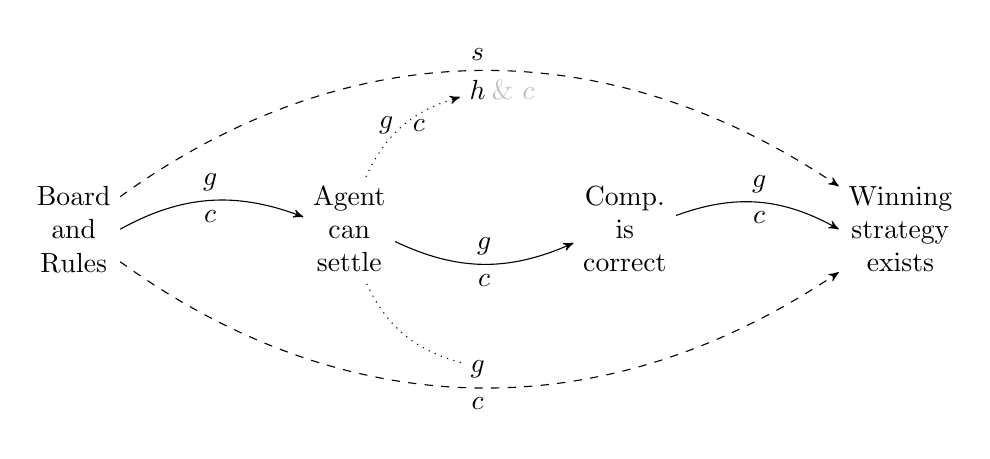
\begin{tikzpicture}[
  ->,
  >=stealth',
  % auto,
  node distance=0cm, every text node part/.style={align=center},
  ]

  \node (1) [] {Board \\ and \\ Rules};
  \node (2) [right of=1, xshift=3.5cm] {Agent \\ can \\ settle};
  \node (3) [right of=2, xshift=3.5cm] {Comp.\ \\ is \\ correct};
  \node (4) [right of=3, xshift=3.5cm] {Winning \\ strategy \\ exists};

  % \draw [->] (1.0) to [bend right=25] (2.180);
  % \draw [->] (2.0) to [bend left=25] (3.180);
  % \draw [->] (3.0) to [bend right=25] (4.180);

  \draw [->] (1.0) to [bend left=25] node[below] {\(c\)} node[above] {\(g\)} (2.165);
  \draw [->] (2.345) to [bend right=25] node[below] {\(c\)} node[above] {\(g\)} (3.195);
  \draw [->] (3.15) to [bend left=25] node[below] {\(c\)} node[above] {\(g\)} (4.180);

  \draw [dashed, ->] (1) to [bend left=35] node[below] (bSH) {\(h \)} node[above] (aSH) {\(s\)} (4);
  \node (x) [right of=bSH, xshift=.45cm, opacity=.25] {\(\&\mbox{ }c\)};
  % \draw [dotted, ->] (1) to [bend left=70] node[below] (bSC) {\(c\)} node[above] {\(s\)} (4);
  \draw [dashed, ->] (1) to [bend right=35] node[below] {\(c\)} node[above] (aGC) {\(g\)} (4);

  \draw [dotted, ->] (2) to [bend left=25] node[right] {\(c\)} node[left] {\(g\)} (bSH);
  % \draw [dotted, ->] (aSH) to [bend right=5] (bSC);
  \draw [dotted, -] (aGC) to [bend left=25] (2);
\end{tikzpicture}
\caption{Main relations}
\label{fig:dynamics}
\end{figure}

Roughly, there's a straightforward general categorical route to the agent's confidence that a winning strategy exists, but this also provides general categorical support for specific hypothetical support that a winning strategy exists.

\subsection{Notes}
\label{sec:notes}

So, what's important here is that there's a different \emph{type} of support available to the agent.
Namely, specific hypothetical (and likely categorical) support as opposed to general categorical support.

The role of the companion is to provide the agent with general categorical support that there is a winning strategy given the state of the board and the rules of chess.
And, after the agent establishes that there is general categorical support for a winning strategy given the state of the board and the rules of chess, it is this together with the agent's confidence that they are able to settle the question of whether there is a winning strategy which provides general categorical support for there being specific hypothetical support for the existence of a winning strategy given the board and the rules of chess.

The importance of the companion is, then, limited.
For example, there is potential for the companion to be providing testimony to the agent.
Yet, the scenario could be recast such that the companion is a somewhat limited computer program or any other instantiation of a random variable with the appropriate statistical properties (i.e.\ agreement with the agent's pattern of settling).
Of course, it may be the case that testimony is provided by the only plausible instantiations of random variables with the appropriate statistical properties, but even if testimony can be appealed to, I doubt that this resolves the puzzle.
For, even if the companion provides testimony that a winning strategy exists, it remains the case that the agent is confident that they are able to reason to the existence of a winning strategy independently of the companions (assumed) testimony.


\section{Inspector Morse and Sergeant Lewis}
\label{sec:second-case}

\begin{note}
  Below is a variation of the chess example that needs a little more work, but which I quite like.
  In short, Morse and Lewis are police officers who share the same powers of deduction and evidence.
  Lewis is a sergeant to Morse's role as inspector, but no longer wishes to enact Morse's commands.

  Lewis is the agent, Morse the companion, and Morse provides Lewis with the information that someone is a suspect given the evidence available to both Morse and Lewis.
  Lewis notices the suspect, and has no interest in approaching the person merely on the basis on Morse thinking that the person is a suspect.
  However, Lewis would approach the person if Lewis thought they were a suspect.
  Hence, given Morse's information about what Lewis could reason to, Lewis ends up approaching the person as a suspect.
\end{note}

Unlike Sherlock and Watson or Marple and a companion, Morse and Lewis are equally matched.\nolinebreak
\footnote{There is a lot that could be said about Morse and Lewis, but for background here a relevant detail is that the dynamic between Morse and Lewis is that of chance and privilege.}

Morse and Lewis have been working on a case together, share the same capacity to reason from evidence, and have examined the same evidence.
Lewis, as a sergeant, has been burdened with other tasks, and Morse is being recalcitrant.
In addition, Lewis has no interest in following Morse's orders.
The police stated is well staffed, and if Morse needs something to be done, and officer (other than Lewis) can be found.
However, Lewis will not refuse to perform a task if More thinks it needs to be done, Lewis' position is against performing a task that Lewis does not recognise as required by their role as a sergeant.

Lewis notices a message on their answer machine when returning home after work.
The message is from Morse who, given the lack of any new information, has been thinking about the case Morse and Lewis have been working on and thinks that it would be worthwhile for Person X to be brought in for questioning, but Morse does not explain why.
The unstated implication of Morse's message is that Lewis should bring Person X in for question tomorrow.
Lewis is confident that it would be worthwhile for Person X to be bought in for questioning, and that Lewis would arrive at this conclusion were they not so overburdened.
Still, bringing Person X in for questioning is a task that any officer could perform, so Lewis is under no pressure to seek Person X --- so tomorrow Lewis will explain to Morse that there are other officers at the police station.

Lewis' position, then, recognises that Morse thinks it is worthwhile for Person X to be brought in for questioning and that Lewis is in a position to recognise that it would be worthwhile for Person X to be bought in for questioning given the information available to Lewis.

The next morning, Lewis is on their way to work and notices Person X in the corner shop.
One the one hand, Lewis can radio in to the police station the location of a suspect that Morse would like to question.
One the other hand, Lewis is confident that they would have, were they to have thought more about the case, formed interest in questioning Person X themselves and Lewis recognises a requirement to themselves bring in for questioning suspects that they would like to question.
So, one the one hand Lewis' requirement is merely to inform the station that Person X has been sighted, while on the other hand Lewis' requirement would be to approach Person X themselves were they recognise the interest in questioning Person X.

Not much thinking is required, and Lewis approaches Person X, frustrated that they have not yet put together when they are interested in questioning Person X, but confident that they are not merely carrying out a task Morse thinks needs to be done.

\section{Middlemarch}
\label{sec:middlemarch}

% \begin{note}
%   I searched through Middlemarch for passages mentioning Pianos, and what follows is the only passage that seemed similar to the kind of cases I've been thinking about.

%   However, I'm not sure that this quite works.
%   For, it's not clear that Rosamond has any reason to think that Ladislaw's coming will require Lydgate to make plans to move to London.
%   Instead, it seems as though Rosamond desires to go to London, but needs some cause for this to happen and Ladislaw's coming could be a cause, and (in a very Humean way) the constant conjunction of these two things in Rosamond's mind lead Rosamond to establish a relation of cause and effect that isn't supported by any particular reasons (though as Eliot notes, this kind of thing wouldn't be unique to Rosamond).

%   Perhaps there's more to the story, though!
%   It could be that Ladislaw is interested in Rosamond, Rosamond recognises this, but hasn't been able to identify the particular dynamic between Ladislaw and Lydgate which would lead Lydgate to make plans for London, but is confident given her general understanding of interpersonal relations that such a dynamic exists.
%   Still, after reading through a few synopsis I'm not sure that this is the case\dots at the very least Rosamond here provides a nice contrast case.
% \end{note}

% \begin{quote}
%   The next day Lydgate had to go to Brassing, and told Rosamond that he should be away until the evening.
%   Of late she had never gone beyond her own house and garden, except to church, and once to see her papa, to whom she said,
%   ``If Tertius goes away, you will help us to move, will you not, papa?
%   I suppose we shall have very little money.
%   I am sure I hope some one will help us.''
%   And Mr.\ Vincy had said,
%   ``Yes, child, I don't mind a hundred or two.
%   I can see the end of that.''
%   With these exceptions she had sat at home in languid melancholy and suspense, fixing her mind on Will Ladislaw's coming as the one point of hope and interest, and associating this with some new urgency on Lydgate to make immediate arrangements for leaving Middlemarch and going to London, till she felt assured that the coming would be a potent cause of the going, without at all seeing how.
%   This way of establishing sequences is too common to be fairly regarded as a peculiar folly in Rosamond.
%   And it is precisely this sort of sequence which causes the greatest shock when it is sundered: for to see how an effect may be produced is often to see possible missings and checks; but to see nothing except the desirable cause, and close upon it the desirable effect, rids us of doubt and makes our minds strongly intuitive.
%   That was the process going on in poor Rosamond, while she arranged all objects around her with the same nicety as ever, only with more slowness---or sat down to the piano, meaning to play, and then desisting, yet lingering on the music stool with her white fingers suspended on the wooden front, and looking before her in dreamy ennui.
%   Her melancholy had become so marked that Lydgate felt a strange timidity before it, as a perpetual silent reproach, and the strong man, mastered by his keen sensibilities towards this fair fragile creature whose life he seemed somehow to have bruised, shrank from her look, and sometimes started at her approach, fear of her and fear for her rushing in only the more forcibly after it had been momentarily expelled by exasperation.\linebreak
%   \mbox{}\hfill\mbox{(Chapter LXXVII.)}
% \end{quote}

\begin{note}
  A little more searching, and I think I have found the passage!
\end{note}

\begin{quote}
  Rosamond played admirably.
  Her master at Mrs.\ Lemon's school (close to a county town with a memorable history that had its relics in church and castle) was one of those excellent musicians here and there to be found in our provinces, worthy to compare with many a noted Kapellmeister in a country which offers more plentiful conditions of musical celebrity.
  Rosamond, with the executant's instinct, had seized his manner of playing, and gave forth his large rendering of noble music with the precision of an echo.
  It was almost startling, heard for the first time.
  A hidden soul seemed to be flowing forth from Rosamond's fingers; and so indeed it was, since souls live on in perpetual echoes, and to all fine expression there goes somewhere an originating activity, if it be only that of an interpreter.
  Lydgate was taken possession of, and began to believe in her as something exceptional.
  After all, he thought, one need not be surprised to find the rare conjunctions of nature under circumstances apparently
  unfavorable: come where they may, they always depend on conditions that are not obvious.
  He sat looking at her, and did not rise to pay her any compliments, leaving that to others, now that his admiration was deepened.\nolinebreak
  \mbox{}\hfill\mbox{(Chapter XVI.)}
\end{quote}

\newpage

\section{Lord}
\label{sec:lord}

\begin{note}
  \citeauthor{Lord:2018aa}'s account of correctly responding to reasons seems a plausible account of what the agent fails to do in the chess scenario.
  For, the state of the board, the agent's grasp of the rules, and the agent's confidence that they can settle on whether there is a winning strategy suggest that the agent possesses reasons to believe that a winning strategy exists.

  However, as \citeauthor{Lord:2018aa} ties correctly responding to reasons to being rational, the agent in the chess example is irrational.
  Further, the agent is irrational even if they merely reason to general categorical support that there is a winning strategy given their confidence that they can settle on whether there is a winning strategy and the reliability of the companion, as it seems the agent possesses specific hypothetical (and categorical) reasons to believe that a winning strategy exists.
\end{note}

\begin{quote}
  You are \emph{ex ante} rational to believe that \emph{p} just in case \emph{p} is supported by sufficient justifiers.
  However, this isn't enough to have an \emph{ex post} rational belief that \emph{p}.
  In order to have an \emph{ex post} rational belief, there must be an appropriate connection between your belief and the justifiers of the belief.\nolinebreak
  \mbox{}\hfill\mbox{(\citeyear[70]{Lord:2018aa})}
\end{quote}

\begin{quote}
  [A] token \(\phi\)-ing is \emph{ex post} rational when
  \begin{enumerate*}[label=(\roman*), ref=\roman*.]
  \item one possesses normative reasons to \(\phi\) that are sufficiently weighty, and
  \item one \(\phi\)-s for those reasons.
  \end{enumerate*}
  \nolinebreak
  \mbox{}\hfill\mbox{(\citeyear[10]{Lord:2018aa})}
\end{quote}

\begin{quote}
  \textbf{Composite Possession}: What it is for agent \emph{A} to possess reason \emph{r} provided by fact \emph{f} to \(\phi\) is for
  \begin{enumerate*}[label=(\roman*), ref=\roman*.]
  \item\label{lord:posession:epistemic} \emph{A} to be in a position to know \emph{f} and
  \item\label{lord:posession:manifest} \emph{A} to be in a position to manifest knowledge about how to use \emph{r} to \(\phi\).
  \end{enumerate*}
  \nolinebreak
  \mbox{}\hfill\mbox{(\citeyear[123]{Lord:2018aa})}
\end{quote}

Strictly speaking, \citeauthor{Lord:2018aa} endorses `Possession', on the basis that condition \ref{lord:posession:epistemic} of `Composite Possession' is a background condition on possession.

\begin{quote}
  \textbf{Possession}: What it is for agent \emph{A} to possess reason \emph{r} to \(\phi\) provided by fact \emph{f} is for \emph{A} to be in a position to manifest knowledge about how to use \emph{r} to \(\phi\).
\end{quote}

\begin{quote}
  \textbf{Possession Enables Rational Routing}: If \emph{A} possesses \emph{r} as a sufficient reason to \(\phi\), then there is a route that \emph{A} can take to \emph{ex post} rational \(\phi\)-ing on the basis of \emph{r}.\nolinebreak
  \mbox{}\hfill\mbox{(\citeyear[100]{Lord:2018aa})}
\end{quote}

Key idea is that \citeauthor{Lord:2018aa} argues for is that the epistemic condition is insufficient as an account of reason possession and that the practical condition fills this gap.

This, seems right, to the extent that we focus on the agent's understanding of the board and the rules of chess it does not seem that the agent possess a reason for confidence that there is a winning strategy.
Instead, it is the combination (or the fulfilment of the background condition) of the agent's understanding of the board and the rules of chess \emph{with} the agent's confidence that the are in a position to use the board and their grasp of the rules of chess which suggests that the agent possesses a reason independently of the companion's answer for confidence that there is a winning strategy.

\begin{quote}
  \textbf{Normative}: \emph{A} \(\phi\)s for a normative reason \emph{r} just in case \emph{A} \(\phi\)s in virtue of the fact that \emph{r} is a normative reason to \(\phi\).
\end{quote}

\begin{quote}
  \textbf{Normative–Sustaining}: \emph{A} \(\phi\)s for a normative reason r if \emph{A} is disposed to revise her \(\phi\)-ing if r ceases to be a normative reason to \(\phi\).\nolinebreak
  \mbox{}\hfill\mbox{(\citeyear[138]{Lord:2018aa})}
\end{quote}

\begin{quote}
  \textbf{Normative–Production}: \emph{A} \(\phi\)s for a normative reason \emph{r} if \emph{A}'s \(\phi\)-ing is the manifestation of a disposition to \(\phi\) when the fact that constitutes \emph{r} is a normative reason to \(\phi\).\nolinebreak
  \mbox{}\hfill\mbox{(\citeyear[139]{Lord:2018aa})}
\end{quote}

\begin{quote}
  \textbf{Normative–Fleshed Out}: \emph{A} \(\phi\)s in virtue of the fact that \emph{r} is a normative reason to \(\phi\) just in case \emph{A}'s \(\phi\)-ing is produced or sustained by \emph{r} (in the ways specified by Normative–Sustaining and Normative–Production).\nolinebreak
  \mbox{}\hfill\mbox{(\citeyear[139]{Lord:2018aa})}
\end{quote}

\begin{quote}
  \textbf{Manifest}: What it is for \emph{A} to \(\phi\) for a normative reason \emph{r} is for \emph{A}'s \(\phi\)-ing to be a manifestation of \emph{A}'s knowledge about how to use \emph{r} as the reason it is to \(\phi\).\nolinebreak
  \mbox{}\hfill\mbox{(\citeyear[139]{Lord:2018aa})}
\end{quote}

\citeauthor{Lord:2018aa} takes `Manifest' to be an account of what it is to react for a normative reason.
\citeauthor{Lord:2018aa} argues, however, is that rationality is guarantee only if an agent's reactions are supported by sufficiently strong normative reasons.
(\citeyear[141]{Lord:2018aa})

\citeauthor{Lord:2018aa} provides the following account of reacting to a sufficient normative reason.

\begin{quote}
  \textbf{Sufficient Normative}: \emph{A} \(\phi\)s for a sufficient normative reason \emph{r} just in case \emph{A} \(\phi\)s in virtue of the fact that \emph{r} is a sufficient normative reason to \(\phi\).\nolinebreak
  \mbox{}\hfill\mbox{(\citeyear[142]{Lord:2018aa})}
\end{quote}

The key here is the `in virtue of' relation, understood through two requirements of an agent's dispositions.

\begin{quote}
  \textbf{Sufficient Normative–Sustaining}: \emph{A} \(\phi\)-s for a sufficient normative reason \emph{r} if \emph{A} is disposed to cease \(\phi\)-ing when \emph{r} ceases to be a sufficient normative reason to \(\phi\).\nolinebreak
  \mbox{}\hfill\mbox{(\citeyear[142]{Lord:2018aa})}
\end{quote}

\begin{quote}
  \textbf{Sufficient Normative–Production}: \emph{A} \(\phi\)s for a sufficient normative reason \emph{r} if \emph{A}'s \(\phi\)-ing is the manifestation of a disposition to \(\phi\) when the fact that constitutes \emph{r} is a sufficient normative reason to \(\phi\).\nolinebreak
  \mbox{}\hfill\mbox{(\citeyear[142]{Lord:2018aa})}
\end{quote}

\citeauthor{Lord:2018aa} suggests that the disjunction of sustaining and manifesting forms a necessary and sufficient condition fir reacting for a sufficient normative reason.

\begin{quote}
  \textbf{Sufficient Normative–Fleshed Out}: \emph{A} \(\phi\)s for a sufficient normative reason \emph{r} just in case \emph{A}'s \(\phi\)-ing is sustained or produced by the fact that \emph{r} is a sufficient normative reason to \(\phi\).\nolinebreak
  \mbox{}\hfill\mbox{(\citeyear[143]{Lord:2018aa})}
\end{quote}

For \citeauthor{Lord:2018aa} reacting to sufficient normative reasons is understood in terms of know-how, leading to:

\begin{quote}
  \textbf{Manifest Sufficient}: What it is for \emph{A} to \(\phi\) for a sufficient normative reason to \(\phi\) is for \emph{A} to manifest knowledge about how to use \emph{r} as the sufficient reason it is to \(\phi\).\nolinebreak
  \mbox{}\hfill\mbox{(\citeyear[143]{Lord:2018aa})}
\end{quote}

This, then completes \citeauthor{Lord:2018aa}'s account of \emph{ex post} rationality.

\begin{quote}
  \textbf{Correctly Responding}: What it is for \emph{A}'s \(\phi\)-ing to be \emph{ex post} rational is for \emph{A} to possess sufficient reason \emph{S} to \(\phi\) and for \emph{A}'s \(\phi\)-ing to be a manifestation of knowledge about how to use \emph{S} as sufficient reason to \(\phi\).\nolinebreak
  \mbox{}\hfill\mbox{(\citeyear[143]{Lord:2018aa})}
\end{quote}

So, in \citeauthor{Lord:2018aa}'s terminology it seems the agent is in a position to be \emph{ex post} rational confidence that there is a winning strategy given the board and the agent's grasp of the rules of chess.
However, the agent does not manifest the appropriate knowledge of how to use the board and the rules of chess to demonstrate the existence of a winning strategy, and hence the agent is not \emph{ex post} rational.

This seems plausible to me.
Of course, there are details that matter, but in broad strokes it is the agent's failure to reason from the board and their grasp of the rules which is striking, and if the agent were to respond to their possessed reasons by reasoning to a winning strategy, then there doesn't seem to be anything particularly interesting about the scenario.
Still, if the agent does not correctly respond to the possessed reasons for a winning strategy, then the agent is not rational on \citeauthor{Lord:2018aa} account, and this is somewhat unsatisfying.



A further question is whether, on \citeauthor{Lord:2018aa}'s account, there is pressure for the agent to believe that there is a winning strategy based on their confidence that they can settle on an answer to whether there is a winning strategy.
\citeauthor{Lord:2018aa} notes three relevant principles.

\begin{quote}
  \textbf{Belief Schema}: If the set of reasons you possess decisively supports \emph{p}, then you are rationally required to believe that \emph{p}.\nolinebreak
  \mbox{}\hfill\mbox{(\citeyear[28]{Lord:2018aa})}
\end{quote}

\begin{quote}
  \textbf{Closure Transmission}: If the reasons you possess decisively support \emph{p} and the reasons you possess decisively support if \emph{p} then \emph{q}, then the reasons you possess decisively support \emph{q}.
\end{quote}

\begin{quote}
  \textbf{Reasons-Coherence, Closure}: If you are closure incoherent, then you are not correctly responding to all of the reasons you possess.
\end{quote}

\citeauthor{Lord:2018aa}'s account of possession limits the scope of Closure/Coherence, as the agent must be able to manifest knowledge about how to use the reason.
This means that it doesn't apply to cases such as the preface paradox, as the condition does not require coherence between arbitrary collections of attitudes.
Still, this does not exclude the chess case, as plausibly it is the case that the reasons the agent possesses do decisively support believing that there is a winning strategy.

The relevant problem is that the agent should recognise that they do not satisfy coherence by `merely' having the required attitude.
Coherence, on \citeauthor{Lord:2018aa}'s view, is a result of correct responsiveness, and so does not seem as though the agent should worry about closure if they recognise that they have not correctly responded to the reasons in their possession.

So, it does not seem that, on \citeauthor{Lord:2018aa}'s account the agent is under pressure to believe that there is a winning strategy given the state of the board and the rules of chess, as the relevant form of irrationality is the failure of the agent to correctly respond to the reasons that they possess.

In part, this can be seen by \citeauthor{Lord:2018aa}'s argument for Reasons-Coherence, Closure.

\begin{quote}
  Reasons-Coherence, Closure is true because it will either be true that you possess decisive reason to believe \emph{p}, decisive reason to believe if \emph{p} then \emph{q} and thus by Closure Transmission possess decisive reason to believe \emph{q}, or you won't.
  If you do possess decisive reason to believe \emph{p}, decisive reason to believe if \emph{p} then \emph{q}, then you'll possess decisive reason to believe \emph{q}, and thus you are irrational when closure incoherent because you don't believe \emph{q}.
  If you lack decisive reason to believe \emph{p} or lack decisive reason to believe if \emph{p} then \emph{q}, then you will be irrational when closure incoherent because you hold one of those beliefs and you are rationally required not to.
  Either way, you will be irrational when closure incoherent.
\end{quote}

Here, \citeauthor{Lord:2018aa} identifies the irrationality of being closure incoherent in terms of failing to correctly respond to possessed reasons.
Therefore, as the agent has not (yet, at least) responding to their possessed reasons in the chess scenario, the agent is irrational, and moreover there is no clear explanation for why the agent would (incorrectly) respond to their possessed reasons as there is no route to rationality other than by correctly responding to their reasons.

% \newpage

% \section{Awake at night}
% \label{sec:awake-at-night}

% Heck, there's something about these kinds of cases that keeps me up at night.
% Because these kinds of parallels suggest that I should be confident that I have some problematic attitudes.
% The contrast is that I don't know what the result of reasoning from these attitudes would be.
% At least these aren't genuine reasons, though.

\section{Further Research}
\label{sec:further-research}

\subsection{Ecological rationality}
\label{sec:ecol-rati}

Two ways to understand ecological rationality.
\begin{enumerate}
\item Providing distinct notion of rationality which is tied to the environment of an agent.
\item Providing a bridge between ideal rationality and an agent situated in an environment.
\end{enumerate}


\newpage

\printbibliography


\end{document}
